\documentclass[a4paper,11pt]{article}
\usepackage{amsmath,amsthm,amsfonts,amssymb,amscd,amstext,vmargin,graphics,graphicx,tabularx,multicol} 
\usepackage[francais]{babel}
\usepackage[utf8]{inputenc}  
\usepackage[T1]{fontenc} 
\usepackage{pstricks-add,tikz,tkz-tab,variations}
\usepackage[autolanguage,np]{numprint} 

\setmarginsrb{1.5cm}{0.5cm}{1cm}{0.5cm}{0cm}{0cm}{0cm}{0cm} %Gauche, haut, droite, haut
\newcounter{numexo}
\newcommand{\exo}[1]{\stepcounter{numexo}\noindent{\bf Exercice~\thenumexo} : \marginpar{\hfill /#1}}
\reversemarginpar


\newcounter{enumtabi}
\newcounter{enumtaba}
\newcommand{\q}{\stepcounter{enumtabi} \theenumtabi.  }
\newcommand{\qa}{\stepcounter{enumtaba} (\alph{enumtaba}) }
\newcommand{\initq}{\setcounter{enumtabi}{0}}
\newcommand{\initqa}{\setcounter{enumtaba}{0}}

\newcommand{\be}{\begin{enumerate}}
\newcommand{\ee}{\end{enumerate}}
\newcommand{\bi}{\begin{itemize}}
\newcommand{\ei}{\end{itemize}}
\newcommand{\bp}{\begin{pspicture*}}
\newcommand{\ep}{\end{pspicture*}}
\newcommand{\bt}{\begin{tabular}}
\newcommand{\et}{\end{tabular}}
\renewcommand{\tabularxcolumn}[1]{>{\centering}m{#1}} %(colonne m{} centrée, au lieu de p par défault) 
\newcommand{\tnl}{\tabularnewline}

\newcommand{\trait}{\noindent \rule{\linewidth}{0.2mm}}
\newcommand{\hs}[1]{\hspace{#1}}
\newcommand{\vs}[1]{\vspace{#1}}

\newcommand{\N}{\mathbb{N}}
\newcommand{\Z}{\mathbb{Z}}
\newcommand{\R}{\mathbb{R}}
\newcommand{\C}{\mathbb{C}}
\newcommand{\Dcal}{\mathcal{D}}
\newcommand{\Ccal}{\mathcal{C}}
\newcommand{\mc}{\mathcal}

\newcommand{\vect}[1]{\overrightarrow{#1}}
\newcommand{\ds}{\displaystyle}
\newcommand{\eq}{\quad \Leftrightarrow \quad}
\newcommand{\vecti}{\vec{\imath}}
\newcommand{\vectj}{\vec{\jmath}}
\newcommand{\Oij}{(O;\vec{\imath}, \vec{\jmath})}
\newcommand{\OIJ}{(O;I,J)}

\newcommand{\bmul}[1]{\begin{multicols}{#1}}
\newcommand{\emul}{\end{multicols}}

\newcommand{\reponse}[1][1]{%
\multido{}{#1}{\makebox[\linewidth]{\rule[0pt]{0pt}{20pt}\dotfill}
}}

\newcommand{\titre}[5] 
% #1: titre #2: haut gauche #3: bas gauche #4: haut droite #5: bas droite
{
\noindent #2 \hfill #4 \\
#3 \hfill #5

\vspace{-1.6cm}

\begin{center}\rule{6cm}{0.5mm}\end{center}
\vspace{0.2cm}
\begin{center}{\large{\textbf{#1}}}\end{center}
\begin{center}\rule{6cm}{0.5mm}\end{center}
}



\begin{document}




\exo

\bmul{2}
Convertir les nombres suivants dans l'unité demandée :\\

13,80 m  = \textcolor{red}{1 380}  cm \\

45 mm  = \textcolor{red}{0,045}  m \\

24,5 km  = \textcolor{red}{245 000}  dm \\

6 372 dam  = \textcolor{red}{63,72}  km \\

\columnbreak

 Compléter avec l'unité qui convient :\\
 
500 dm  =   50 \textcolor{red}{m} \\

0,7 dm  =    7  \textcolor{red}{cm}  \\

0,09 dam  =   90 \textcolor{red}{cm} \\

500 000 m  =   500 \textcolor{red}{km}\\ 


\emul

\textbf{Exercice 2}\\

\bmul{2}

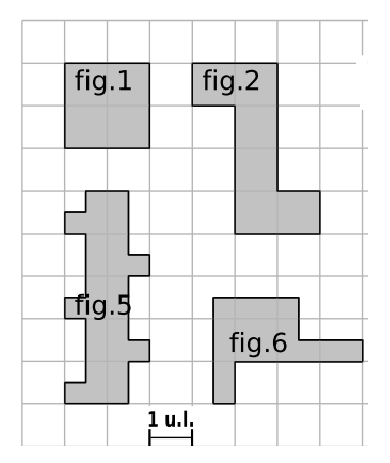
\includegraphics[scale=0.8]{figperimetrecompte.eps} 

\columnbreak

Observer   attentivement   l'unité   de   longueur (1 u.l.) puis déterminer le périmètre, en unités de longueur, de chaque figure.\\

\color{red}

$P_{fig1} = 8 $ u. l.  \hspace*{1cm} $P_{fig2} = 14 $ u. l. \\

$P_{fig5} = 17 $ u. l.  \hspace*{1cm} $P_{fig6} = 12 $ u. l. \\

\color{black}
\emul

\vspace*{1.5cm}

\textbf{Exercice 3}\\

\q Calculer le périmètre d'un rectangle MLKJ tel que ML = 9 m et LK = 5,3 m. \\

\color{red}

Les longueurs sont bien dans la même unité, on peut donc utiliser la formule :\\

 $P_{rect}= (l+L) \times 2$\\
 
$P_{rect}= (9 + 5,3) \times 2$\\

$P_{rect}= 14,3 \times 2$\\

\fbox{$P_{rect}= 28,6$ m}\\

\color{black}
\q Calculer le périmètre d'un carré OLKI tel que OL = 7,5 cm.  \\

\color{red}

$P_{carre}= 4 \times c$\\
 
$P_{carre}= 4 \times 7,5 $\\


\fbox{$P_{carre}= 30$ cm}\\


\color{black}
\

\textbf{Exercice 4 :}

Calculer le périmètre des figures suivantes : \\

\bmul{2}

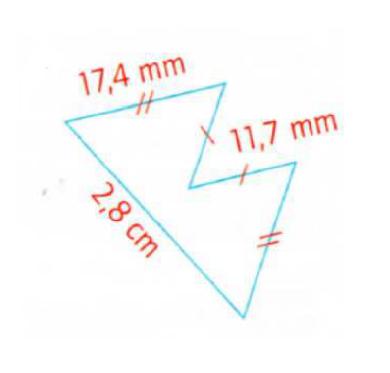
\includegraphics[scale=0.7]{fig1perimetre.eps} \\

\color{red}

La figure est un polygone, on va donc additionner toutes ses longueurs.\\

Je vérifie d'abord que toutes les longueurs sont exprimées dans la même unité :\\

2,8 cm = 28 mm.\\

 $P_{Fig1}= (17,4 \times 2) + (11,7 \times 2 ) + 28$\\
 
  $P_{Fig1}= 34,8 + 23,4 + 28$\\

\fbox{$P_{Fig1}= 86,2$ mm}\\

\color{black}


\columnbreak

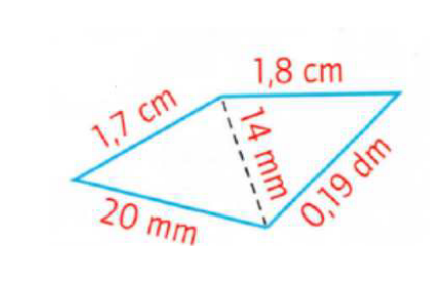
\includegraphics[scale=0.7]{fig2perimetre.eps} \\

\color{red}

La figure est un polygone, on va donc additionner toutes ses longueurs.\\

Je vérifie d'abord que toutes les longueurs sont exprimées dans la même unité :\\

20 mm = 2 cm \hspace*{1cm} 0,19 dm = 1,9 cm\\

 $P_{Fig2}= 1,7 + 1,8 + 2 + 1,9$\\
 
\fbox{$P_{Fig2}= 7,4$ cm}\\

\color{black}

\emul

\textbf{Exercice 5}\\
Calculer le périmètre des figures suivantes : 

\bmul{2}
\textbf{FIGURE 1}\\
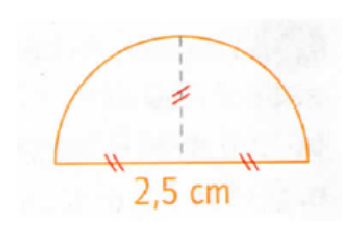
\includegraphics[scale=0.8]{fig4.eps} 

\columnbreak

\textbf{FIGURE 2}\\
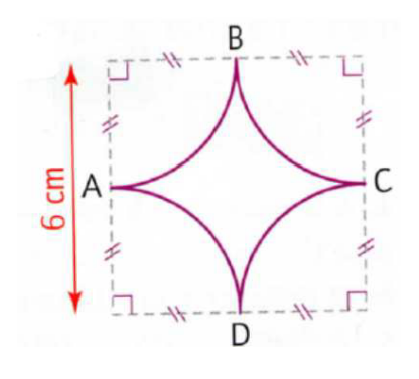
\includegraphics[scale=0.7]{fig4perimetre.eps} 


\emul

\color{red}

\textbf{FIGURE 1} \\
La figure est composée d'un segment de 2,5 cm et d'un demi-cercle de diamètre 2,5 cm.\\

- Le   demi-cercle : \\

Pour calculer le demi-cercle, on calcule d'abord le périmètre d'un cercle et on le divise par 2 ensuite.\\


$P_{cercle} =  \pi \times d $\\

$P_{cercle} =  \pi \times 2,5 $\\

$P_{cercle} \approx  3,14 \times 2,5 $\\

$P_{cercle} \approx 7,85$ cm\\

$P_{demi-cercle}= \dfrac{P_{cercle}}{2}$ \\

$P_{demi-cercle} \approx \dfrac{7,85}{2}$ \\

$P_{demi-cercle} \approx 3,925$ cm\\

- On additionne ensuite toutes les longueurs qui composent la figure :\\

$P_{TOTAL} = P_{segment} + P_{demi-cercle} $\\

$P_{TOTAL} \approx 2,5 + 3,925 $\\

\fbox{$P_{TOTAL} \approx 6,425 $ cm} \\

\textbf{FIGURE 2} \\
La figure est composée de 4 quarts de cercle de rayon 3 cm.\\
Si je rassemble les 4 quarts de cercle de \textbf{même rayon}, j'obtiens un cercle de rayon 3 cm.\\



- Le   cercle : \\


$P_{cercle} = 2 \times \pi \times r $\\

$P_{cercle} = 2 \times \pi \times 3 $\\

$P_{cercle} \approx 2 \times 3,14 \times 3 $\\

\fbox{$P_{cercle} \approx 18,84$ cm} \hspace*{1cm} Le périmètre de la figure 2 est de 18,84 cm.\\


\color{black}

\textbf{Exercice 6 :} Calculer le périmètre de la figure suivante :

\begin{center}
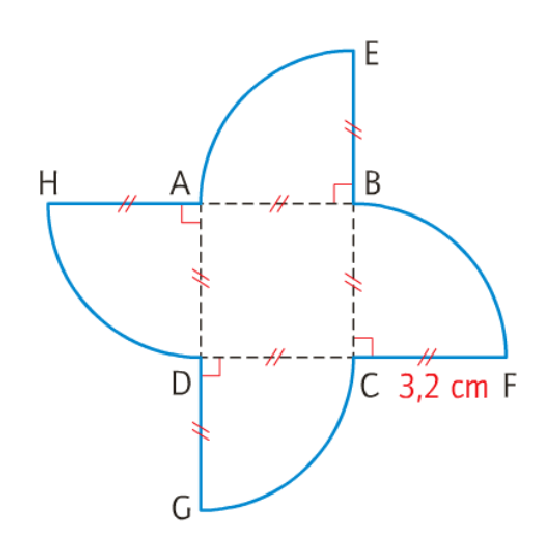
\includegraphics[scale=0.6]{fig6.eps} 
\end{center}

\color{red}

La figure est composée de 4 segments de même longueur et de 4 quarts de cercle de rayon 3,2 cm.\\
Si je rassemble les 4 quarts de cercle de \textbf{même rayon}, j'obtiens un cercle de rayon 3,2 cm.\\


- Les segments :\\

$P_{segments} = 4 \times 3,2$\\

$P_{segments} = 12,8 $ cm\\





- Le   cercle : \\


$P_{cercle} = 2 \times \pi \times r $\\

$P_{cercle} = 2 \times \pi \times 3,2 $\\

$P_{cercle} \approx 2 \times 3,14 \times 3,2 $\\

$P_{cercle} \approx 20,096$ cm\\



- On additionne ensuite toutes les longueurs qui composent la figure :\\

$P_{TOTAL} = P_{segments} + P_{cercle} $\\

$P_{TOTAL} \approx 12,8 + 20,096 $\\

\fbox{$P_{TOTAL} \approx 32,896 $ cm} \\


\end{document}
